\chapter{Selection - \keyword{If} and \keyword{Select}}
	\label{ch:selection}

	This chapter explains:
	\begin{itemize}
		\item how to use \keyword{If} and \keyword{Select} statements to carry out tests;
		\item how to use operators such as >;
		\item how to use \keyword{And}, \keyword{Or} and \keyword{Not};
		\item how to declare and use \keyword{Boolean} data.
	\end{itemize}

  \section{Introduction}
		We all make selections in daily life. We wear a coat if it is raining. We buy a CD if we have enough money. Selections are also used a lot in programs. The computer tests a value and, according to the result, takes one course of action or another. Whenever the program has a choice of actions and decides to take one action or the other, an \keyword{If} or a \keyword{Select} statement is used to describe the situation.

		We have seen that a computer program is a series of instructions to a computer. The computer obeys the instructions one after another in sequence. But sometimes we want the computer to carry out a test on some data and then take one of a choice of actions depending on the result of the test. For example, we might want the computer to test someone's age and then tell them either that they may vote or that they are too young. This is called selection. It uses a statement (or instruction) called the \keyword{If} statement, the central subject of this chapter.
		
		\keyword{If} statements are so important that they are used in every programming language that has ever been invented.


		\begin{figure}[th]
			\centering
			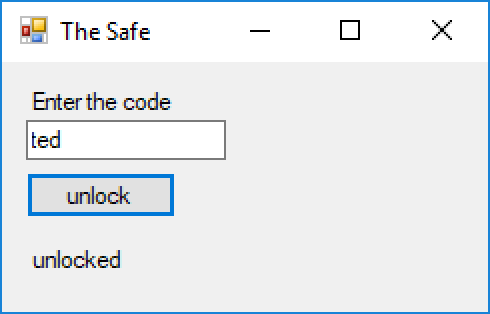
\includegraphics[width=5cm]{selection_safe_screen}
			\caption{Screen for the safe program.}
			\label{fig:selection_safe_screen}
		\end{figure}


  \section{The \keyword{If} statement}
		Our first example is a program that simulates the digital lock on a safe. The screen is as shown in \Vref{fig:selection_safe_screen}. The safe is locked unless the user enters the correct code into a text box. The text box is initially emptied when the form is designed. The program compares the text that is entered with the correct code. If the code is correct, a message is displayed.
		\begin{lstlisting}
Private Sub Button1_Click(sender As System.Object,
		e As System.EventArgs)
		Handles Button1.Click
	Dim code As String
	Label2.Text = ""
	code = TextBox1.Text
	If code = "bill" Then
		Label2.Text = "unlocked"
	End If
End Sub
		\end{lstlisting}
		The \keyword{If} statement tests the value of the string. If the string equals the value 'bill', the statement sandwiched between the \keyword{If} and the \keyword{End If} is carried out. Next, any statement after the \keyword{End If} is executed. On the other hand, if the string is not equal to 'bill', the sandwiched statement is ignored and any statement after the \keyword{End If} is executed.

		\begin{figure}[th]
			\centering
			\begin{tikzpicture}[node distance=2cm]
				\node (start) [startstop] {Begin};
				\node (decision) [decision, below of=start,anchor=center] {Selection};
				\node (h1) [right = 3.5cm of decision] {};
				\node (proc1) [process, align=center] at (decision -| h1) {display\\unlocked};
				\node (stop) [startstop, below = 1.5cm of decision] {End};
	
				\draw [arrow] (start) -- (decision);
				\draw [arrow] (decision) -- node[anchor=east] {[code <> "ted"]} (stop);
				\draw [arrow] (decision) -- node[anchor=south,midway] {[code = "ted"]} (proc1);
				\draw [arrow] (proc1) |- (stop);
			\end{tikzpicture}
			\caption{Flowchart for an \keyword{If} statement.}
			\label{fig:selection_fc1}
	 	\end{figure}

		One way of visualizing an \keyword{If} statement is as a flowchart diagram (\Vref{fig:selection_fc1}). This shows the above \keyword{If} statement in graphical form. To use this diagram, start at the blob at the top and follow the arrows. A decision is shown as a diamond, with the two possible conditions shown in square brackets. Actions are shown in a process boxes and the end of the sequence is a specially shaped blob at the bottom of the diagram.
		
		There are two parts to the \keyword{If} statement:
		\begin{itemize}
				\item the condition being tested;
				\item the statement or sequence of statements to be executed if the condition is true.
		\end{itemize}
		All programs consist of a sequence of actions, and the sequence evident here is:
		\begin{enumerate}
			\item	A piece of text is input from the text box.
			\item Next a test is done.
			\item	If appropriate, a message is displayed to say that the safe is unlocked.
		\end{enumerate}
		Very often we want not just one, but a complete sequence of actions carried out if the result of the test is true, and these are sandwiched between the \keyword{If} statement and the \keyword{End If} statement.
	
		\subsection*{Indentation}
			Notice that the lines are indented to reflect the structure of this piece of program. (Indentation means using spaces to push the text over to the right.) The VB development system does this automatically when you type in an \keyword{If} statement. Although indentation is not essential, it is highly desirable so that the (human) reader of a program can understand it easily. All good programs (whatever the language) have indentation and all good programmers use it.

			\begin{figure}[th]
				\centering
				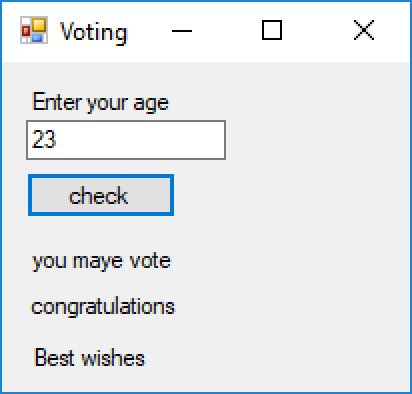
\includegraphics[width=5cm]{selection_voting_screen}
				\caption{The voting checker program screen.}
				\label{fig:selection_voting_screen}
			\end{figure}


		\subsection*{\keyword{If}…\keyword{Else}}
			Sometimes we want to specify two sequences of actions - those that are carried out if the condition is true and those that are carried out if the condition is false.
			
			The user of the voting checker program enters their age into a text box and the program decides whether they can vote or not. The screen is shown in \Vref{fig:selection_voting_screen}. When the user clicks on the button, the program extracts the information that the user has entered into the text box, converts the string into an integer and places the number in the variable called \keyword{age}. Next we want the program to take different actions depending on whether the value is:
			\begin{itemize}
				\item greater than 17, or
				\item less than or equal to 17.
			\end{itemize}
			Then the results of the test are displayed in a number of labels.
			\begin{lstlisting}
Private Sub Button1_Click(sender As System.Object,
		e As System.EventArgs)
		Handles Button1.Click
	Dim age As Integer
	age = CInt(TextBox1.Text)
	If age > 17 Then
		DecisionLabel.Text = "you may vote"
		CommentaryLabel.Text = "congratulations"
	Else
		DecisionLabel.Text = "you may not vote"
		CommentaryLabel.Text = "sorry"
	End If
	SignOffLabel.Text = "Best Wishes"
End Sub
			\end{lstlisting}
			There are three parts to this \keyword{If} statement:
			\begin{itemize}
				\item the condition being tested - in this case whether the age is greater than 17;
				\item the statement or sequence of statements to be executed if the condition is true;
				\item the statement or statements to be executed if the condition is false.
			\end{itemize}
			The new element here is the word \keyword{Else}, which introduces the second part of the \keyword{If} statement. Notice again how the indentation helps to emphasize the intention of the program.
			
			We can visualize an \keyword{If}…\keyword{Else} statement as a flowchart diagram, as shown in \Vref{fig:selection_fc2}. The diagram shows the condition being tested and the two separate actions.

			\begin{figure}[th]
				\centering
				\begin{tikzpicture}[node distance=1cm]
					\node (start) [startstop] {Begin};
					\node (io) [below = of start, io,align=center] {input\\age};
					\node (dec1) [decision, below = of io] {Selection};
					\node (h1) [below = 1cm of dec1] {};
					\node (proc1) [process, align=center, right = of h1] {you may not vote};
					\node (proc2) [process, align=center, left = of h1] {you may vote};
					\node (proc3) [process, below = 1.5cm of h1,align=center] {display\\"best wishes"};
					\node (stop) [startstop,below = of proc3] {End};
	
					\draw [arrow] (start) -- (io);
					\draw [arrow] (io) -- (dec1);
					\draw [arrow] (dec1) -| node[anchor=east] {[age > 17]} (proc2);
					\draw [arrow] (dec1) -| node[anchor=south,midway] {[age <= 17]} (proc1);
					\draw [arrow] (proc1) |- (proc3);
					\draw [arrow] (proc2) |- (proc3);
					\draw [arrow] (proc3) -- (stop);
			\end{tikzpicture}
			\caption{Flowchart for an \keyword{If}…\keyword{Else} statement.}
			\label{fig:selection_fc2}
	 	\end{figure}

  \section{Comparison operators}
		The programs above used some of the comparison operators. Here is a complete list:

		\begin{center}
			\begin{tabular}{ll}
				\toprule Symbol &	Means \\ \midrule
				> & greater than\\
				< & less than\\
				= & equals\\
				<>& not equal to\\
				<=& less than or equal to\\
				>=& greater than or equal to\\ \bottomrule
			\end{tabular}
		\end{center}

		Notice that VB uses the equals sign (=) to test whether two things are equal. This same symbol is also used to assign a value to a variable.

		Choosing the appropriate operator often has to be done with great care. In the program to test whether someone can vote, the appropriate test should probably be:
		\begin{lstlisting}
If age >= 18 Then
	DecisionLabel.Text = "you can vote"
End If
		\end{lstlisting}
		Note that it is usually possible to write conditions in either of two ways. The following two program fragments achieve exactly the same result, but use different conditions:
\begin{lstlisting}
If age >= 18 Then
	DecisionLabel.Text = "you may vote"
Else
	DecisionLabel.Text = "sorry"
End If
\end{lstlisting}
		achieves the same end as:
		\begin{lstlisting}
If age < 18 Then
	DecisionLabel.Text = "sorry"
Else
	DecisionLabel.Text = "you may vote"
End If
		\end{lstlisting}
		Although these two fragments achieve the same end result, the first is probably better, because it spells out more clearly the condition for eligibility to vote.



		\begin{stqb}
			\begin{STQ}
				\item	Do these two pieces of VB achieve the same end or not?
					\begin{lstlisting}
If age > 18 Then
	Label2.Text = "you may vote"
End If
If age < 18 Then
	Label2.Text = "you may not vote"
End If
					\end{lstlisting}
			\end{STQ}
		\end{stqb}


	\section{\keyword{And}, \keyword{Or}, \keyword{Not}}
		Often in programming we need to test two things at once. Suppose, for example, we want to test whether someone should pay a junior rate for a ticket:
		\begin{lstlisting}
If age > 6 And age < 16 Then
	Label1.Text = "junior rate"
End If
		\end{lstlisting}
		The word \keyword{And} is one of the VB logical operators and simply means 'and' as we would use it normal language.

		
		Brackets can be used to improve the readability of these more complex conditions. For example we can rewrite the above statement as:
		\begin{lstlisting}
If (age > 6) And (age < 16) Then
	Label1.Text = "junior rate"
End If
		\end{lstlisting}
		Although the brackets are not essential, they serve to distinguish the two conditions being tested. 
		
		It might be very tempting to write:
		\begin{lstlisting}
If age > 6 And < 18 Then    ' error!
		\end{lstlisting}
		but this is incorrect because the conditions have to be spelled out in full as follows:
		\begin{lstlisting}
If age > 6 And age < 18 Then    ' OK
		\end{lstlisting}
		We would use the \keyword{Or} operator in an \keyword{If} statement like this:
		\begin{lstlisting}
If age < 6 Or age > 60 Then
	Label1.Text = "reduced rate"
End If
		\end{lstlisting}
		in which the reduced rate is applicable for people who are younger than 6 or older than 60.

		The \keyword{Not} operator, with the same meaning as in English, gets a lot of use in programming, even though in English the use of a negative can suffer from lack of clarity. Here is an example of the use of not:
		\begin{lstlisting}
If Not (age > 18) Then
	Label1.Text = "too young"
End If
		\end{lstlisting}
		This means: test to see if the age is greater than 18. If this result is true, make it false. If it is false, make it true. Then, if the outcome is true, display the message. This can, of course, be written more simply without the \keyword{Not} operator.


		\begin{stqb}
			\begin{STQ}
				\item	Rewrite the above \keyword{If} statement without using the \keyword{Not} operator.
			\end{STQ}
		\end{stqb}

		This next program illustrates a more complex series of tests. Two dice are thrown in a betting game and the program has to decide what the result is. We will create two track bars, each with a range of 1 to 6 to specify the values of each of the two dice (\Vref{fig:selection_dice_screen}). To start with, we make the rule that only a total score of six wins anything.

		\begin{figure}[th]
			\centering
			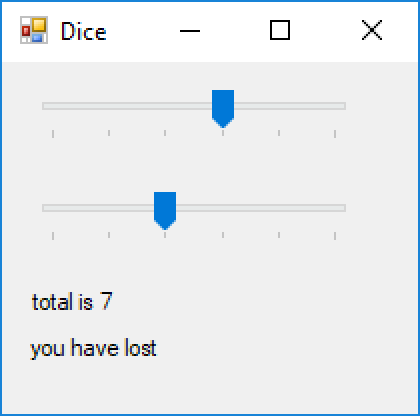
\includegraphics[width=5cm]{selection_dice_screen}
			\caption{The dice program, version 1.}
			\label{fig:selection_dice_screen}
		\end{figure}

		The program code is given below. Whenever either of the two track bars is moved, the method is called to display the total value and decide whether a win has occurred.
		\begin{lstlisting}
Private Sub TrackBar1_Scroll(sender As Object,
		e As System.EventArgs)
		Handles TrackBar1.Scroll
	CheckValues()
End Sub
Private Sub TrackBar2_Scroll(sender As Object,
		e As System.EventArgs)
		Handles TrackBar2.Scroll
	CheckValues()
End Sub
Private Sub CheckValues()
	Dim die1, die2, total As Integer
	die1 = TrackBar1.Value
	die2 = TrackBar2.Value
	total = die1 + die2
	Label1.Text = "total is " & total
	If total = 6 Then
			Label2.Text = "you have won"
	Else
			Label2.Text = "you have lost"
	End If
End Sub
		\end{lstlisting}
		Now we will alter the rules and see how to rewrite the program. Suppose that any pair of identical values wins, i.e. two ones, two twos, etc. Then the \keyword{If} statement is:
		\begin{lstlisting}
If die1 = die2 Then
	Label2.Text = "you have won"
End If
		\end{lstlisting}
		Now let's suppose that you only win if you get a total of either 2 or 7:
		\begin{lstlisting}
If (total = 2) Or (total = 7) Then
	Label2.Text = "you have won"
End If
		\end{lstlisting}
		Notice that we have enclosed each of the conditions with brackets. These brackets aren't strictly necessary in VB, but they help a lot to clarify the meaning of the con-dition to be tested.


		\begin{stqb}*
			\begin{STQ}
				\item	Alter the program so that a win is a total value of 2, 5 or 7.
				\item Write \keyword{If} statements to test whether someone is eligible for full-time employment. The rule is that you must be 16 or above and younger than 65.
			\end{STQ}
		\end{stqb}



	\section{Nested \keyword{If}s and \keyword{ElseIf}}
		Look at the following program fragment:
		\begin{lstlisting}
If age > 6 Then
	If age < 16 Then
		Label1.Text = "junior rate"
	Else
		Label1.Text = "adult rate"
	End If
Else
	Label1.Text = "child rate"
End If
		\end{lstlisting}
		You will see that the second \keyword{If} statement is completely contained within the first. (The indentation helps to make this clear.) This is called \emph{nesting}. Nesting is not the same as indentation - it is just that the indentation makes the nesting very apparent. The meaning of this nested code is as follows:
		\begin{itemize}
			\item If the age is greater than 6, then the second \keyword{If} is carried out.
			\item If the age is not greater than 6, then the \keyword{Else} part is carried out.
		\end{itemize}
		The overall effect of this piece of program is:
		\begin{itemize}
			\item If the age is greater than 6 and less than 16, the rate is the junior rate.
			\item If the age is greater than 6 but not less than 16, the rate is the adult rate.
			\item If the age is not greater than 6, the rate is the child rate.
		\end{itemize}
		It is common to see nesting in programs, but a program like this has a complexity which makes it slightly difficult to understand. Often it is possible to write a program more simply using the logical operators and/or a variation of the \keyword{If} statement that uses \keyword{ElseIf}. Here, for example, the same result as above is achieved without nesting:
		\begin{lstlisting}
If (age > 6) And (age < 16) Then
	Label1.Text = "junior rate"
ElseIf age >= 16 Then
	Label1.Text = "adult rate"
Else
	Label1.Text = "child rate"
End If
		\end{lstlisting}
		The \keyword{If}…\keyword{ElseIf} statement describes a series of mutually exclusive choices. The first condition follows the initial \keyword{If}. Subsequent conditions follow any number of \keyword{ElseIf} keywords. Optionally there is a final \keyword{Else} to address any condition that has not already been met. There is a single \keyword{End If} at the end of the complete statement.

		We now have two pieces of program that achieve the same end result, one with nesting and one without. Some people argue that it is hard to understand nesting, such a program is prone to errors and that therefore nesting should be avoided. Nesting can always be avoided using either logical operators or \keyword{ElseIf} or both.

		\begin{stqb}
			\begin{STQ}
				\item	Write a program to input a salary from a track bar and determine how much tax someone should pay according to the following rules:
					\begin{quote}
People pay no tax if they earn up to \$10 000. They pay tax at the rate of 20\% on the amount they earn over \$10 000 but up to \$50 000. They pay tax at 90\% on any money they earn over \$50 000. The track bar should have a range from 0 to 100 000.
					\end{quote}
			\end{STQ}
		\end{stqb}

		In the next program we create two track bars, labelled as Rick and Morty. The program compares the values and reports on which one is set to the larger value. The screen is shown in \Vref{fig:selection_rick_and_morty_screen}. The library method \keyword{FillRectangle} is used to draw a solid rectangle whose width across the screen is equal to the value obtained from the corresponding track bar.

			\begin{figure}[th]
				\centering
				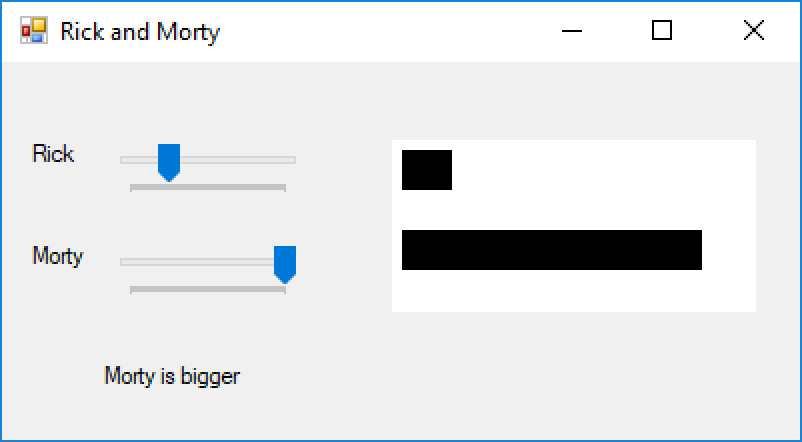
\includegraphics[width=8cm]{selection_rick_and_morty_screen}
				\caption{Screen for the Rick and Morty program.}
				\label{fig:selection_rick_and_morty_screen}
			\end{figure}


				\begin{lstlisting}
Private Sub TrackBar1_Scroll(sender As Object,
		e As System.EventArgs)
		Handles TrackBar1.Scroll
	CompareValues()
End Sub
Private Sub TrackBar2_Scroll(sender As Object,
		e As System.EventArgs)
		Handles TrackBar2.Scroll
	CompareValues()
End Sub
Private Sub CompareValues()
	Dim paper As Graphics
	paper = PictureBox1.CreateGraphics()
	Dim myBrush As New SolidBrush(Color.Black)
	Dim mortyValue, rickValue As Integer
	rickValue = TrackBar1.Value
	mortyValue = TrackBar2.Value
	paper.Clear(Color.White)
	paper.FillRectangle(myBrush, 10, 10, rickValue, 20)
	paper.FillRectangle(myBrush, 10, 50, mortyValue, 20)
	If rickValue > mortyValue Then
		Label1.Text = "Rick is bigger"
	Else
		Label1.Text = "Morty is bigger"
	End If
End Sub
		\end{lstlisting}
		This program works fine, but again illustrates the importance of care when you use \keyword{If} statements. In this program, what happens when the two values are equal? The answer is that the program finds that Morty is bigger - which is clearly not the case. We could enhance the program to spell things out more clearly by changing the \keyword{If} statement to:
		\begin{lstlisting}
If mortyValue > rickValue Then
	Label1.Text = "Morty is bigger"
ElseIf rickValue > mortyValue Then
	Label1.Text = "Rick is bigger"
Else
	Label1.Text = "They are equal"
End If
		\end{lstlisting}
		This is another illustration of an \keyword{If} statement with an \keyword{ElseIf} part.

		\begin{stqb}
			\begin{STQ}
				\item	Write a program that creates three track bars and displays the largest of the three values.
			\end{STQ}
		\end{stqb}

		This next example is a program that keeps track of the largest value of a number as it changes. Some stereo amplifiers have a display that shows the volume being created. The display waxes and wanes according to the volume at any point in time. Sometimes the display has an indicator that shows the maximum value that is currently being output. This program displays the numerical value of the maximum value that the track bar is set to (see \Vref{fig:selection_amplifier_screen}). It uses a single \keyword{If} statement that compares the current value of the track bar with the value of a variable named \keyword{max}, a class-level variable that holds the value of the largest value achieved so far. \keyword{max} is declared like this:

		
			\begin{figure}[th]
				\centering
				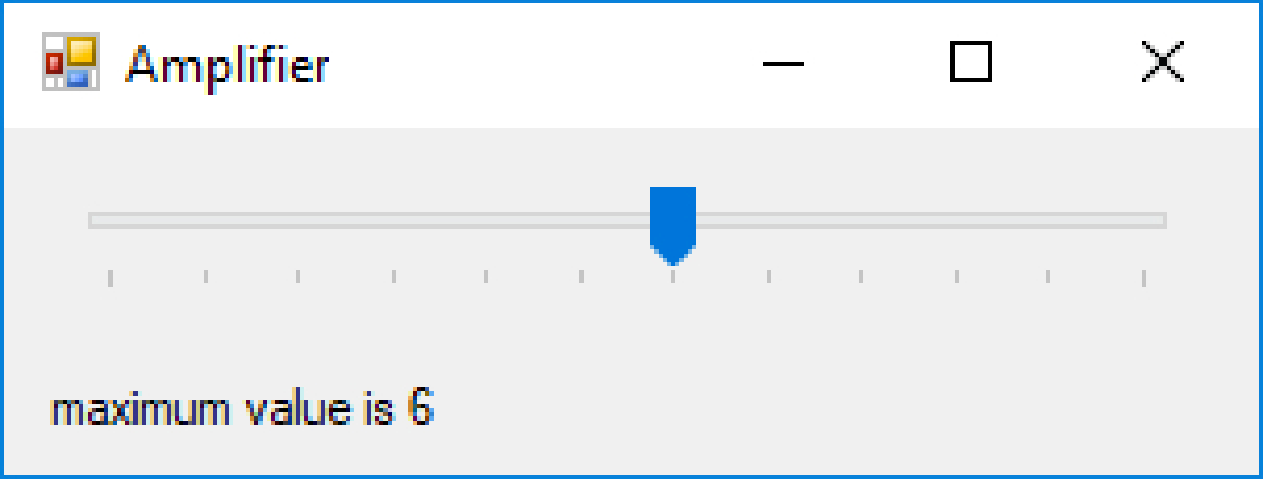
\includegraphics[width=6cm]{selection_amplifier_screen}
				\caption{Screen for the amplifier display.}
				\label{fig:selection_amplifier_screen}
			\end{figure}


		\begin{lstlisting}
Private max As Integer = 0
and the method to handle track bar events is:
Private Sub TrackBar1_Scroll(sender As Object,
		e As System.EventArgs)
		Handles TrackBar1.Scroll
	Dim volume As Integer
	volume = TrackBar1.Value
	If volume > max Then
		max = volume
	End If
	Label1.Text = "maximum value is " & CStr(max)
End Sub
		\end{lstlisting}

		\begin{stqb}*
			\begin{STQ}
				\item	Write a program that displays the numerical value of the minimum value that the track bar is set to.
				\item The Young and Beautiful holiday company restricts its clients to ages between 18 and 30. (Below 18 you have no money; after 30 you have too many wrinkles.) Write a program to test whether you are eligible to go on holiday with this company.
			\end{STQ}
		\end{stqb}

		We now return to the dice-throwing program discussed earlier. Instead of inputting the dice values via the track bars, we change the program so that the computer decides the die values randomly. We will create a button, labelled 'throw'. When it is clicked, the program will obtain two random numbers and use them as the die values (\Vref{fig:selection_gambling_screen}).

			\begin{figure}[th]
				\centering
				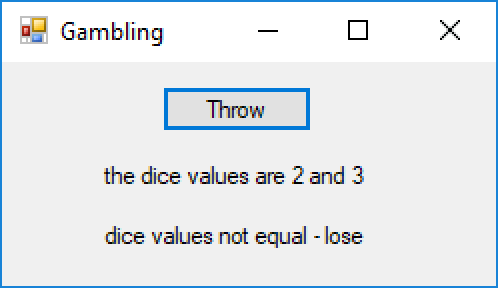
\includegraphics[width=5cm]{selection_gambling_screen}
				\caption{The dice program, version 2.}
				\label{fig:selection_gambling_screen}
			\end{figure}


		To get a random number in VB, we create an object from the library class \keyword{Random} and then use its method \keyword{Next}. This method returns a random number, an \keyword{Integer} in any range we choose, specified by the parameters. We met this class back in \Cref{ch:objects}.
		
		The program to throw two dice is given below. At class level we declare:
		\begin{lstlisting}
Private randomNumber As Random = New Random()
		\end{lstlisting}
		and then the event-handling method is:
		\begin{lstlisting}
Private Sub Button1_Click(sender As Object,
		e As System.EventArgs)
		Handles Button1.Click
	Dim die1, die2 As Integer
	die1 = randomNumber.Next(1, 6)
	die2 = randomNumber.Next(1, 6)
	Label1.Text = "the die values are "
		& CStr(die1) & " and " & CStr(die2)
	If die1 = die2 Then
		Label2.Text = "dice equal - a win"
	Else
		Label2.Text = "dice not equal - lose"
	End If
End Sub
		\end{lstlisting}


	\section{\keyword{Select}}
		The \keyword{Select} statement is another way of doing a lot of \keyword{If} statements. You can always accomplish everything you need with the aid of \keyword{If} statements but \keyword{Select} can be useful in appropriate circumstances. For example, suppose we need a piece of program to display the day of the week as a string. Suppose that the program represents the day of the week as an \keyword{Integer} variable called \keyword{dayNumber}, which has one of the values 1 to 7, representing the days Monday to Sunday. We want to convert the integer version of the day into a string version called \keyword{dayName}. We could write the following series of \keyword{If} statements:
		\begin{lstlisting}
If dayNumber = 1 Then
	dayName = "Monday"
ElseIf dayNumber = 2 Then
	dayName = "Tuesday"
ElseIf dayNumber = 3 Then
	dayName = "Wednesday"
ElseIf dayNumber = 4 Then
	dayName = "Thursday"
ElseIf dayNumber = 5 Then
	dayName = "Friday"
ElseIf dayNumber = 6 Then
	dayName = "Saturday"
ElseIf dayNumber = 7 Then
	dayName = "Sunday"
End If
		\end{lstlisting}
		Now although this piece of coding is neat, clear and well-structured, there is an alternative that has the same effect using the \keyword{Select} statement:
\begin{lstlisting}
Select Case dayNumber
	Case 1
		dayName = "Monday"
	Case 2
		dayName = "Tuesday"
	Case 3
		dayName = "Wednesday"
	Case 4
		dayName = "Thursday"
	Case 5
		dayName = "Friday"
	Case 6
		dayName = "Saturday"
	Case 7
		dayname = "Sunday"
End Select
\end{lstlisting}
		This now exploits the symmetry of what needs to happen more clearly than the equivalent series of \keyword{ElseIf}s. Notice that the complete \keyword{Select} statement ends with a \keyword{End Select} statement.

		A \keyword{Select} statement like this can be visualized as an activity diagram in \Vref{fig:selection_fc3}.


		\begin{figure}[th]
			\centering
				\begin{tikzpicture}[node distance=1.5cm]
					\node (start) [startstop] {Begin};
					\node (dec1) [decision, below = of start] {Selection};
					\node (proc1) [process, align=center, left = of dec1] {display\\"Monday"};
					\node (proc2) [process, align=center, below = of dec1] {display\\"Thursday"};
					\node (proc3) [process, right =of dec1, align=center] {display\\"Sunday"};
					\node (stop) [startstop,below = of proc2] {End};
	
					\draw [arrow] (start) -- (dec1);
					\draw [arrow] (dec1) -- node[anchor=west] {[day = 4]}  (proc2);
					\draw [arrow] (dec1) -- node[anchor=south] {[day = 1]}  (proc1);
					\draw [arrow] (dec1) -- node[anchor=south] {[day = 7]}  (proc3);
					\draw [arrow] (proc1) |- (stop);
					\draw [arrow] (proc2) -- (stop);
					\draw [arrow] (proc3) |- (stop);
			\end{tikzpicture}
			\caption{Flowchart for a \keyword{Select} statement.}
			\label{fig:selection_fc3}
	 	\end{figure}

		\begin{stqb}
			\begin{STQ}
				\item	Write a method that converts the integers 1, 2, 3 and 4 into the words diamonds, hearts, clubs and spades respectively.
			\end{STQ}
		\end{stqb}

		Several statements can follow one of the options in a \keyword{Select} statement. For example, one of the options could be:
		\begin{lstlisting}
Case 6
	MessageBox.Show("hurray")
	dayName = "Saturday"
		\end{lstlisting}
Another feature of the \keyword{Select} statement is grouping several options together, like this:
\begin{lstlisting}
Select Case dayNumber
Case 1, 2, 3, 4, 5
	dayName = "weekday"
Case 6, 7
	dayName = "weekend"
End Select
\end{lstlisting}
		Another, sometimes useful, part of the \keyword{Select} statement is the \keyword{Else} option. Suppose in the above example that the value of the integer denoting the day of the week is input from a text box. Then there is the distinct possibility that the user will erroneously enter a number that is not in the range 1 to 7. Any decent program needs to take account of this, in order to prevent something odd happening or the program crashing. The \keyword{Select} statement is very good at dealing with this situation, because we can supply a 'catch-all' or default option that will be used if none of the others are valid:
		\begin{lstlisting}
Select Case dayNumber
	Case 1
		dayName = "Monday"
	Case 2
		dayName = "Tuesday"
	Case 3
		dayName = "Wednesday"
	Case 4
		dayName = "Thursday"
	Case 5
		dayName = "Friday"
	Case 6
		dayName = "Saturday"
	Case 7
		dayName = "Sunday"
	Case Else
		dayName = "illegal day"
End Select
		\end{lstlisting}
		If an \keyword{Else} option is not written as part of a \keyword{Select} statement and if none of the cases provided corresponds to the actual value of the variable, then all the options are ignored.

		The \keyword{Select} statement is very useful, but unfortunately it is not as flexible as it could be. Suppose, for example, we want to write a piece of program to display two numbers, with the larger first, followed by the smaller. Using \keyword{If} statements, we would write:
		\begin{lstlisting}
If a > b Then
	Label1.Text = CStr(a) & " is greater than " & CStr(b)
ElseIf b > a Then
	Label1.Text = CStr(b) & " is greater than " & CStr(a)
Else
	Label1.Text = "they are equal"
End If
		\end{lstlisting}
		We may be tempted to rewrite this using a \keyword{Select} statement as follows:
		\begin{lstlisting}
Select Case ? ' beware! illegal VB
	Case a > b
		Label1.Text = CStr(a) & " is greater than" & CStr(b)
	Case b > a
		Label1.Text = CStr(b) & " is greater than" & CStr(a)
	Case a = b
		Label1.Text = "they are equal"
End Select
		\end{lstlisting}
		but this is not allowed because, as indicated by the question mark, \keyword{Select} only works with a single integer or string variable as its subject, and \keyword{Case} cannot use >, <, etc.


		\begin{figure}[th]
			\centering
			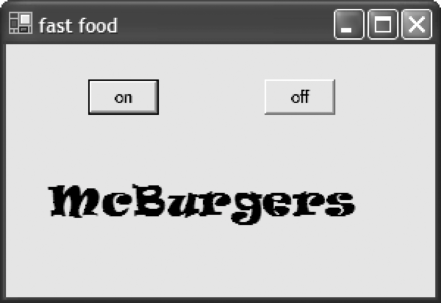
\includegraphics[width=5cm]{selection_boolean_sign}
			\caption{The sign, switched using \keyword{Boolean} values.}
			\label{fig:selection_boolean_sign}
		\end{figure}


	\section{Boolean variables}
		All of the types of variable that we have met so far are designed to hold numbers or strings. Now we meet a new kind of variable called a \keyword{Boolean}, that can only hold either the value \keyword{True} or the value \keyword{False}. The words \keyword{Boolean}, \keyword{True} and \keyword{False} are reserved keywords in VB and cannot be used for any other purpose. This type of variable is named after the 19th-century British mathematician George Boole who made a large contribution towards the development of mathematical logic, in which the ideas of true and false play a central role.

		We will introduce \keyword{Boolean} variables by looking at the properties of the labels that are available from the toolbox. \Vref{fig:selection_boolean_sign} shows a display that can either be switched on or switched off using buttons. When the user clicks on the buttons the \keyword{Visible} property of the label is changed:
		\begin{lstlisting}
Private Sub OffButton_Click(sender As Object,
		e As System.EventArgs)
		Handles OffButton.Click
	Label1.Visible = False
End Sub
Private Sub OnButton_Click(sender As Object,
		e As System.EventArgs)
		Handles OnButton.Click
	Label1.Visible = True
End Sub
		\end{lstlisting}
		The \keyword{Visible} property is a \keyword{Boolean} and we can change the value as shown above. We can also test its value using \keyword{If} statements. So we could rewrite the program so that it has a single button that switches the display from visible to invisible, or vice versa, using the statements:
		\begin{lstlisting}
Private Sub Button1_Click(sender As Object,
		e As System.EventArgs)
		Handles Button1.Click
	If Label1.Visible = True Then
		Label1.Visible = False
	Else
		Label1.Visible = True
	End If
End Sub
		\end{lstlisting}
		Now that we have seen how to use a \keyword{Boolean} property, we next look at declaring our own \keyword{Boolean} variables. We can declare a variable of type \keyword{Boolean} like this:
		\begin{lstlisting}
Dim finished As Boolean
		\end{lstlisting}
		and we can assign either of the values True and False, as in:
		\begin{lstlisting}
finished = True
		\end{lstlisting}
		Equally importantly, we can test the value of a \keyword{Boolean} in an \keyword{If} statement, for example:
		\begin{lstlisting}
If finished Then
	MessageBox.Show("Good bye")
End If
		\end{lstlisting}
		The value of \keyword{finished} is tested, and if it is True the accompanying statement is executed. An equivalent, but slightly more cumbersome, way of writing the same test is:
		\begin{lstlisting}
If finished = True Then
	MessageBox.Show("Good bye")
End If
		\end{lstlisting}
		\keyword{Boolean} variables are used in programming to remember something, perhaps for a short time, perhaps for the whole time that the program is running. As an example, we look at a program, \Vref{fig:selection_remember_screen}, that draws a rectangle in a picture box when a button is clicked. Sometimes we want the rectangle to be drawn in outline and sometimes we want it drawn filled in. We provide two buttons allowing the user to specify their option. Once a button has been clicked, the program remembers the option until the user clicks again on a button.
		
		The class-level declaration of the \keyword{Boolean} variable is:
		\begin{lstlisting}
Private filled As Boolean = True
		\end{lstlisting}
		This is the variable that remembers what the user has specified. It either has the value \keyword{True} (to denote that rectangles should be filled in) or it has the value \keyword{False}.
		
		
		\begin{figure}[th]
			\centering
			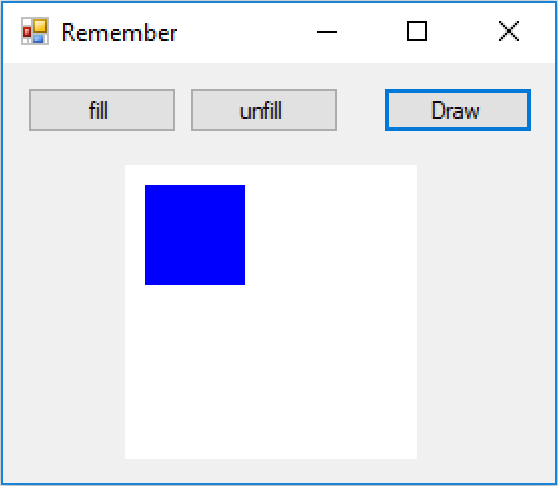
\includegraphics[width=5cm]{selection_remember_screen}
			\caption{The display from the remember program.}
			\label{fig:selection_remember_screen}
		\end{figure}


		The methods to handle button-clicks simply make the \keyword{Boolean} \keyword{True} or \keyword{False} as appropriate:
		\begin{lstlisting}
Private Sub FillButton_Click(sender As Object,
		e As System.EventArgs)
		Handles FillButton.Click
	filled = True
End Sub
Private Sub UnFillButton_Click(sender As Object,
		e As System.EventArgs)
		Handles UnFillButton.Click
	filled = False
End Sub
		\end{lstlisting}
		When the user clicks on the \ui{draw} button, the program first tests the value of the \keyword{Boolean} value filled using an \keyword{If} statement and then either draws a filled or an unfilled rectangle.
		\begin{lstlisting}
Private Sub DrawButton_Click(sender As Object,
			e As System.EventArgs)
			Handles DrawButton.Click
	Dim paper As Graphics = PictureBox1.CreateGraphics()
	Dim myPen As Pen = New Pen(Color.Black)
	Dim myBrush As SolidBrush = New SolidBrush(Color.Black)
	paper.Clear(Color.White)
	If filled = True Then
		paper.FillRectangle(myBrush, 10, 10, 50, 50)
	Else
		paper.DrawRectangle(myPen, 10, 10, 50, 50)
	End If
End Sub
		\end{lstlisting}
		Methods can use \keyword{Boolean} values as parameters and as return values. For example, here is a method that checks whether three numbers are in numerical order:
		\begin{lstlisting}
Private Function InOrder(a as Integer,
			b As Integer,
			c As Integer) As Boolean
	If (a <= b) And (b <= c) Then
		Return True
	Else
		Return False
	End If
End Sub
		\end{lstlisting}


  \section{Programming principles}
	The computer normally obeys instructions one-by-one in a sequence. An \keyword{If} statement instructs the computer to test the value of some data and then take one of a choice of actions depending on the result of the test. This choice is sometimes called \emph{selection}. The test of the data is called a \emph{condition}. After an \keyword{If} statement is completed, the computer continues obeying the instructions in sequence.


	\section{Programming pitfalls}
		You might find that you have written an \keyword{If} statement like this:
		\begin{lstlisting}
If a > 18 And < 25 Then
		\end{lstlisting}
		which is wrong. Instead, the \keyword{And} must link two complete conditions, preferably in brackets for clarity, like this:
		\begin{lstlisting}
If (a > 18) And (a < 25) Then
		\end{lstlisting}

	\section{Grammar spot}
		The first kind of \keyword{If} statement has the structure:
		\begin{lstlisting}
If condition Then
	statements
End If
		\end{lstlisting}
		The second type of \keyword{If} statement has the structure:
		\begin{lstlisting}
If condition Then
	statements
Else
	statements
End If
		\end{lstlisting}
		The third type of \keyword{If} statement has the structure that follows this pattern:
		\begin{lstlisting}
If condition Then
	statements
ElseIf condition Then
	statements
ElseIf condition Then
	statements
Else
	statements
End If
		\end{lstlisting}
		The final \keyword{Else} is optional.
		
		The \keyword{Select} statement has the structure:
		\begin{lstlisting}
Select Case variable
	Case value1
		statements
	Case value2
		statements
	Case Else
		statements
End Select
		\end{lstlisting}
		The final \keyword{Case Else} is optional.

	\section{New language elements}
		\begin{itemize}
			\item Control structures for decisions: \keyword{If}, Then, \keyword{ElseIf}, \keyword{Else}, \keyword{End If}, \keyword{Select}, \keyword{Case}, \keyword{Else}, \keyword{Select}
			\item The comparison operators >, <, =, <>, <= and >=
			\item The logical operators \keyword{And} \keyword{Or} \keyword{Not}
			\item Variables declared as \keyword{Boolean}, which can take either the value \keyword{True} or the value \keyword{False}.
		\end{itemize}


	\section{Summary}
		\begin{itemize}
			\item \keyword{If} statements allow the programmer to control the sequence of actions by making the program carry out a test. Following the test, the computer carries out one of a choice of actions.
			\item There are three varieties of \keyword{If} statement:
				\begin{lstlisting}
If . . . Then . . . End If
If . . . Then . . . Else . . . End If
If . . . Then . . . ElseIf . . . End If
				\end{lstlisting}
			\item A \keyword{Boolean} variable can be assigned the value \keyword{True} or the value \keyword{False}. A \keyword{Boolean} variable can be tested with an \keyword{If} statement.
			\item The \keyword{Select} statement provides a convenient way of carrying out a number of tests. However, the \keyword{Select} statement is restricted to tests on integers or on strings.
		\end{itemize}
	
	\section{Exercises}
		\begin{EXE}
			\item	\name{Deal a card} Write a program with a single button on it which, when clicked, randomly selects a single playing card. First use the random number generator in the library to create a number in the range 1 to 4. Then convert the number to a suit (heart, diamond, club, spade). Next use the random number generator to create a random number in the range 1 to 13. Convert the number to an ace, 2, 3, etc. and finally display the value of the chosen card. (Hint: use \keyword{Select} as appropriate.)
			\item \name{Sorting} Write a program to input numbers from three track bars, or three text boxes, and display them in increasing numerical size.
			\item \name{Cinema (movie theatre) price} Write a program to work out how much a person pays to go to the cinema. The program should input an age from a track bar or a text box and then decide on the following basis:
				\begin{itemize}
					\item under 5, free;
					\item aged 5 to 12, half price;
					\item aged 13 to 54, full price;
					\item aged 55, or over, free.
				\end{itemize}
			\item \name{Betting} A group of people are betting on the outcome of three throws of the dice. A person bets \$1 on predicting the outcome of the three throws. Write a program that uses the random number method to simulate three throws of a die and displays the winnings according to the following rules:
				\begin{itemize}
					\item all three throws are sixes: win \$20;
					\item all three throws are the same (but not sixes): win \$10;
					\item any two of the three throws are the same: win \$5.
				\end{itemize}
			\item	\name{Digital combination safe} Write a program to act as the digital combination lock for a safe. Create three buttons, representing the numbers 1, 2 and 3. The user clicks on the buttons, attempting to guess the correct numbers (say 331121). The program remains unhelpfully quiet until the correct buttons are pressed. Then it congratulates the user with a suitable message. A button is provided to allow users to restart.
			
				Enhance the program so that it has another button which allows the user to change the safe's combination.
			\item	\name{Rock, scissors, paper game} In its original form, each of the two players simultaneously chooses one of rock, scissors or paper. Rock beats scissors, paper beats rock and scissors beats paper. If both players choose the same, it is a draw. Write a program to play the game. The player selects one of three buttons, marked rock, scissors or paper. The computer makes its choice randomly using the random number generator. The computer also decides and displays who has won.
			\item	\name{The calculator} Write a program which simulates a simple desk calculator (\Vref{fig:selection_calculator_screen}) that acts on integer numbers. It has one button for each of the 10 digits, 0 to 9. It has a button to add and a button to subtract. It has a clear button, to clear the display, and an equals (=) button to get the answer.

			  When the clear button is pressed, the display is set to zero and the (hidden) total is set to zero.

			  When a digit button is pressed, the digit is added to the right of those already in the display (if any).

			  When the + button is pressed, the number in the display is added to the total (and similarly for the - button).

			  When the = button is pressed, the value of the total is displayed.

			
		\begin{figure}[th]
			\centering
			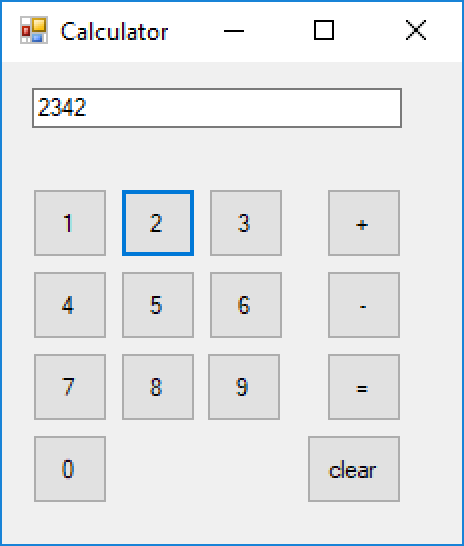
\includegraphics[width=5cm]{selection_calculator_screen}
			\caption{The calculator.}
			\label{fig:selection_calculator_screen}
		\end{figure}

			\item	\name{The elevator} Write a program to simulate a very primitive elevator. The elevator is represented as a filled rectangle. There are two buttons - one to make it move up the screen and one to make it move down.
			\item \name{Nim} is a game played with matchsticks (unused or used, it does not matter). It doesn't matter how many matches there are. The matches are put into three piles. Again, it doesn't matter how many matches there are in each pile. Each player goes in turn. A player can remove any number of matches from any one pile, but only one pile. A player must remove at least one match. The winner is the person who causes the other player to take the last match.
				Write a program to play the game. Initially the computer deals three piles, with a random number (in the range 1 to 200) of matches in each pile. One player is the computer, which chooses a pile and an amount randomly. The other player is the human user, who specifies the pile number and quantity using text boxes, before clicking on a 'go' button.
			\item	\name{Turtle graphics} Turtle graphics is a way of making programming easy for young children. Imagine a pen fixed to the belly of a turtle. As the turtle crawls around a floor, the pen draws on the floor. The turtle can be issued with commands as follows:
				\begin{itemize}
					\item pen up
					\item pen down
					\item turn left 90°
					\item turn right 90°
					\item go forward n pixels
				\end{itemize}
				Initially the turtle is at coordinates 0, 0 and facing to the right.
				So, for example, we can draw a rectangle using the sequence:
				\begin{enumerate}
					\item pen down
					\item go forward 20 pixels
					\item turn right 90°
					\item go forward 20 pixels
					\item turn right 90°
					\item go forward 20 pixels
					\item turn right 90°
					\item go forward 20 pixels
				\end{enumerate}
				Write a program that behaves as the turtle, with one button for each of the commands. The number of pixels, n, to be moved is input via a track bar or a text box.
		\end{EXE}


		\begin{stab}
			\begin{enumChapter}
			
			\item	No, because they treat the particular age of 18 differently.
			\item
				\begin{lstlisting}
If age <= 18 Then
	Label1.Text = "too young"
End If
				\end{lstlisting}
			\item
				\begin{lstlisting}
If (total = 2) Or (total = 5) Or (total = 7) Then
	Label2.Text = "you have won"
End If
				\end{lstlisting}
			\item
				\begin{lstlisting}
If age >= 16 And age < 65 Then
	MessageBox.Show("you are eligible")
End If
				\end{lstlisting}
			\item
				\begin{lstlisting}
Dim salary, tax As Integer
salary = TrackBar1.Value
If (salary > 10000) And (salary <= 50000) Then
	tax = (salary - 10000)/5
ElseIf salary > 50000 Then
	tax = 8000 + ((salary - 50000) * 9 / 10)
Else
	tax = 0
End If
				\end{lstlisting}
			\item 
				\begin{lstlisting}
Dim a, b, c As Integer
a = TrackBar1.Value
b = TrackBar2.Value
c = TrackBar3.Value
If a > b And a > c Then
	largest = a
ElseIf b > a And b > c Then
	largest = b
ElseIf c > a And c > b Then
	largest = c
End If
MessageBox.Show("largest value is " & CStr(largest))
				\end{lstlisting}
			\item	The essential part of this program is:
				\begin{lstlisting}
If volume < min Then
	min = volume
End If
Label2.text = "Minimum value is " & CStr(min)
				\end{lstlisting}

			\item
				\begin{lstlisting}
Dim age As Integer
age = CInt(TextBox1.Text)
If age >= 18 And age <= 30 Then
	TextBox2.Text = "you are eligible"
End If
				\end{lstlisting}
			\item
				\begin{lstlisting}
Function Convert(s As Integer) As String
	Dim suit As String
	Select Case s
		Case 1
			suit = "diamonds"
		Case 2
			suit = "hearts"
		Case 3
			suit = "clubs"
		Case 4
			suit = "spades"
	End Select
	Return suit
End Function
				\end{lstlisting}
			\end{enumChapter}
		\end{stab}

